\section{Method}\label{sec:method}

\subsection{Problem Formulation}

CODA operates on the entire score page. Layout metadata provides a finite set of systems and bars, along with their bounding boxes, for each page. The model selects among candidate systems and bars on the current page.

At each audio frame $t$, let $h_t = (x_{\le t},\, I)$ denote the causal audio history and the score image for the current page. The model predicts three quantities: the active system index $s_t$, the active bar index $b_t$ within that system, and a continuous note position $u_t = (c_x, c_y)$ expressed in bar-local coordinates. Rather than predicting all three independently, CODA factorizes the joint distribution as
\begin{equation}
\begin{split}
p(s_t, b_t, u_t \mid h_t) = {} & p(s_t \mid h_t) \cdot p(b_t \mid s_t, h_t) \\
& \cdot\; p(u_t \mid b_t, s_t, h_t).
\end{split}
\end{equation}
This cascaded factorization enforces valid geometric structure by construction: the predicted bar always lies within the predicted system, and the predicted note always lies within the predicted bar.

\subsection{Model Architecture}

Figure~\ref{fig:overview} illustrates CODA's overall architecture. CODA has two input streams: audio and visual. The audio stream is converted into a 78-dimensional log-filterbank at 20~frames per second. A two-layer causal Mamba encoder~\cite{gu2024mamba} processes each frame. Its recurrent state compactly accumulates the entire audio history up to frame~$t$, yielding a conditioning vector~$z_t$. In parallel, a sliding window $H_t$ of the most recent $L$ per-frame outputs is maintained. $z_t$ provides conditioning for the visual feature map via FiLM, while $H_t$ serves as the key and value source for cross-attention between candidate visual regions and the recent audio history (Section~\ref{sec:cascade}).
 
The visual stream takes the score page image as input. The score page image is processed by a CNN backbone with FiLM conditioning driven by~$z_t$ at deeper stages. The output of the CNN backbone is further processed by a Feature Pyramid Network (FPN) that produces a stride-8 feature map~$F$ (i.e., at one-eighth the spatial resolution of the input). This feature map is shared across all three cascade stages (Section~\ref{sec:cascade}).

\subsection{Cascaded Selection}
\label{sec:cascade}
Given the shared stride-8 feature map~$F$ from the visual input stream and the Mamba encoder outputs from the audio input stream, CODA applies three cascaded stages to localize the active position on the score page. Each stage narrows the spatial scope before proceeding to the next stage. All three stages share a common processing pipeline, with stage-specific variations detailed below. Figure~\ref{fig:tracking} illustrates the output on a real score page: the selected system (green), bar (blue), and note position (red) are each geometrically contained within the previous level.

\begin{figure}[h]
\centering
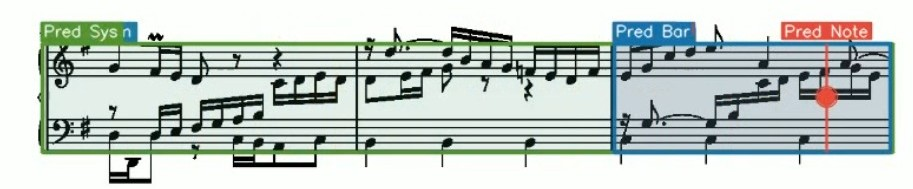
\includegraphics[width=\columnwidth]{figures/CODA.jpg}
\caption{CODA tracking output on an MSMD score page.}
\label{fig:tracking}
\end{figure}

Recall that $H_t \in \mathbb{R}^{L \times d}$ is the sliding window of the most recent $L$ Mamba outputs, with $d$ as the hidden dimension of the encoder. For each candidate region~$r$ (a system or bar bounding box from the score layout metadata), the pipeline proceeds as follows.

First, Region of Interest (ROI) Align \cite{he2017mask} extracts a fixed-size feature patch $f_r = \mathrm{ROIAlign}(F, r)$ from the stride-8 feature map. The extracted features are modulated by the audio vector~$z_t$ via FiLM as $\tilde{f}_r = \gamma(z_t) \odot f_r + \beta(z_t)$, where $\gamma$ and $\beta$ are learned linear projections and $\odot$ denotes element-wise multiplication. Convolutional layers further process the conditioned features: $\hat{f}_r = \mathrm{Conv}(\tilde{f}_r)$. In the system and bar stages, the convolved features are refined by scaled dot-product cross-attention \cite{vaswani2017attention} over the audio buffer: $\bar{f}_r = \mathrm{softmax}\!\left(\mathrm{flat}(\hat{f}_r)\,(W_a H_t)^\top / \sqrt{C}\right) W_a H_t$, where queries are formed by spatially flattening $\hat{f}_r$, keys and values are shared projections of $H_t$, and $W_a$ is a learned linear projection onto the $C$-dimensional attention space shared with $\hat{f}_r$. This cross-attention lets each candidate region attend to fine-grained temporal patterns in the recent audio history.

The system stage applies the full pipeline above (ROI Align, FiLM, convolution, cross-attention) to every system candidate on the page, producing~$\log p(s_t \mid h_t)$ via adaptive average pooling, a linear classifier, and softmax normalization. The bar stage applies the same pipeline with independent parameters to the bars within the selected system, yielding~$\log p(b_t \mid s_t, h_t)$. The note stage applies only ROI Align, FiLM, and convolution (no cross-attention at this stage) on the selected bar and regresses bar-local coordinates~$u_t = (c_x, c_y) \in [0,1]^2$ via sigmoid activation.

\subsection{Beam Search and Temporal Priors}

At each audio frame, the cascaded selection described above produces a log-probability over systems and another log-probability over bars within each system. To decode these scores over time, CODA uses beam search combined with learnable temporal priors.

At each frame~$t$, the model first scores every system on the page and retains the top-$k$ candidates. For each candidate system, the bars within that system are scored, and the top-$m$ candidates are retained per system. The actual values of $k$ and $m$ are specified in Section~\ref{sec:setup}. The note head is evaluated only on the winning system--bar pair after the beam has been resolved. This two-level pruning keeps inference efficient: the full system distribution is computed once per frame, but bar-level and note-level computation is restricted to the $k \times m$ beam.

The beam ranking combines model confidence with learned temporal priors that encode transition preferences between consecutive frames. Specifically, the composite score for a system--bar hypothesis~$(s, b)$ at frame~$t$ is
\begin{equation}
\begin{split}
\mathrm{score}_t(s,b) = {} & \log p(s_t \mid h_t) + \tau_s(s_t, s_{t-1}) \\
& + \log p(b_t \mid s_t, h_t) + \tau_b(b_t, b_{t-1}),
\end{split}
\end{equation}
where $\tau_s$ and $\tau_b$ are page-local transition penalties for systems and bars, respectively. These priors are implemented as learnable parameters that are trained end-to-end with the rest of the model. They are clamped to remain non-positive, with the stay transition (i.e., $s_t = s_{t-1}$ or $b_t = b_{t-1}$) fixed at zero. This parameterization biases the tracker toward smooth temporal progression by encouraging smooth transitions and penalizing large jumps. However, the penalties are bounded rather than hard-coded, so the model can still override them when the audio strongly indicates that a real jump is occurring. The jump detection and recovery mechanism will be covered in Section~\ref{subsec:jump}.

The hypothesis with the highest composite score determines the predicted system~$\hat{s}_t$ and bar~$\hat{b}_t$. The note head then regresses the note position~$\hat{u}_t$ within the selected bar, and the final output is the triplet~$(\hat{s}_t, \hat{b}_t, \hat{u}_t)$.

\subsection{Training}

Because CODA is cascaded, the bar and note stages only consider candidates within the selected system. This cascaded dependency means that if the system prediction is wrong, all downstream predictions will also be wrong. If the model is trained exclusively with ground-truth system labels, it never learns to handle incorrect system inputs, creating a mismatch between training and inference.

To address this, training proceeds in two phases using scheduled sampling~\cite{bengio2015scheduled}. In the first phase, the bar and note stages always receive the ground-truth system labels from training data. This allows the bar head to focus on discriminating among bar candidates under ideal system selections. In the second phase, starting from the first-phase checkpoint, the model's own system prediction is gradually mixed in. At each training step in the second phase, the ground-truth system is replaced by the model's self-predicted system with probability~$p_{\mathrm{pred}}$, which increases linearly from~0 to a maximum value~$p_{\max}$ over training. When the predicted system is wrong and does not contain the ground-truth bar, the bar and note training losses for that frame are masked because there is no meaningful supervision target. The system loss remains active, so the system head continues to receive corrective gradients. This two-phase curriculum training schedule progressively closes the gap between training and inference conditions.

The system and bar stages are trained with cross-entropy loss over their respective candidate sets, and the note head is trained with mean squared error on the bar-local coordinates. The three task losses are combined via learned uncertainty weighting \cite{kendall2018multi}:
\begin{equation}\label{eq:loss}
\mathcal{L} = \frac{1}{2\sigma_s^2}\mathcal{L}_{\mathrm{sys}} + \frac{1}{2\sigma_b^2}\mathcal{L}_{\mathrm{bar}} + \frac{1}{2\sigma_n^2}\mathcal{L}_{\mathrm{note}} + \log \sigma_s \sigma_b \sigma_n,
\end{equation}
where $\sigma_s$, $\sigma_b$, and $\sigma_n$ are learnable task-specific uncertainty parameters that balance the three objectives automatically.

\subsection{Jump Detection and Recovery}
\label{subsec:jump}

Score discontinuities such as repeats, D.C., and coda jumps cause the active position to move non-monotonically. Rather than modeling each type separately, CODA treats all discontinuities as arbitrary position changes preceded by silence. This assumption is grounded in the observation of Nakamura et al.~\cite{nakamura2016real}. This also covers unscripted performer errors. CODA realizes this with two mechanisms demonstrated in Figure~\ref{fig:jump_recovery}.

\begin{figure}[h]
\centering
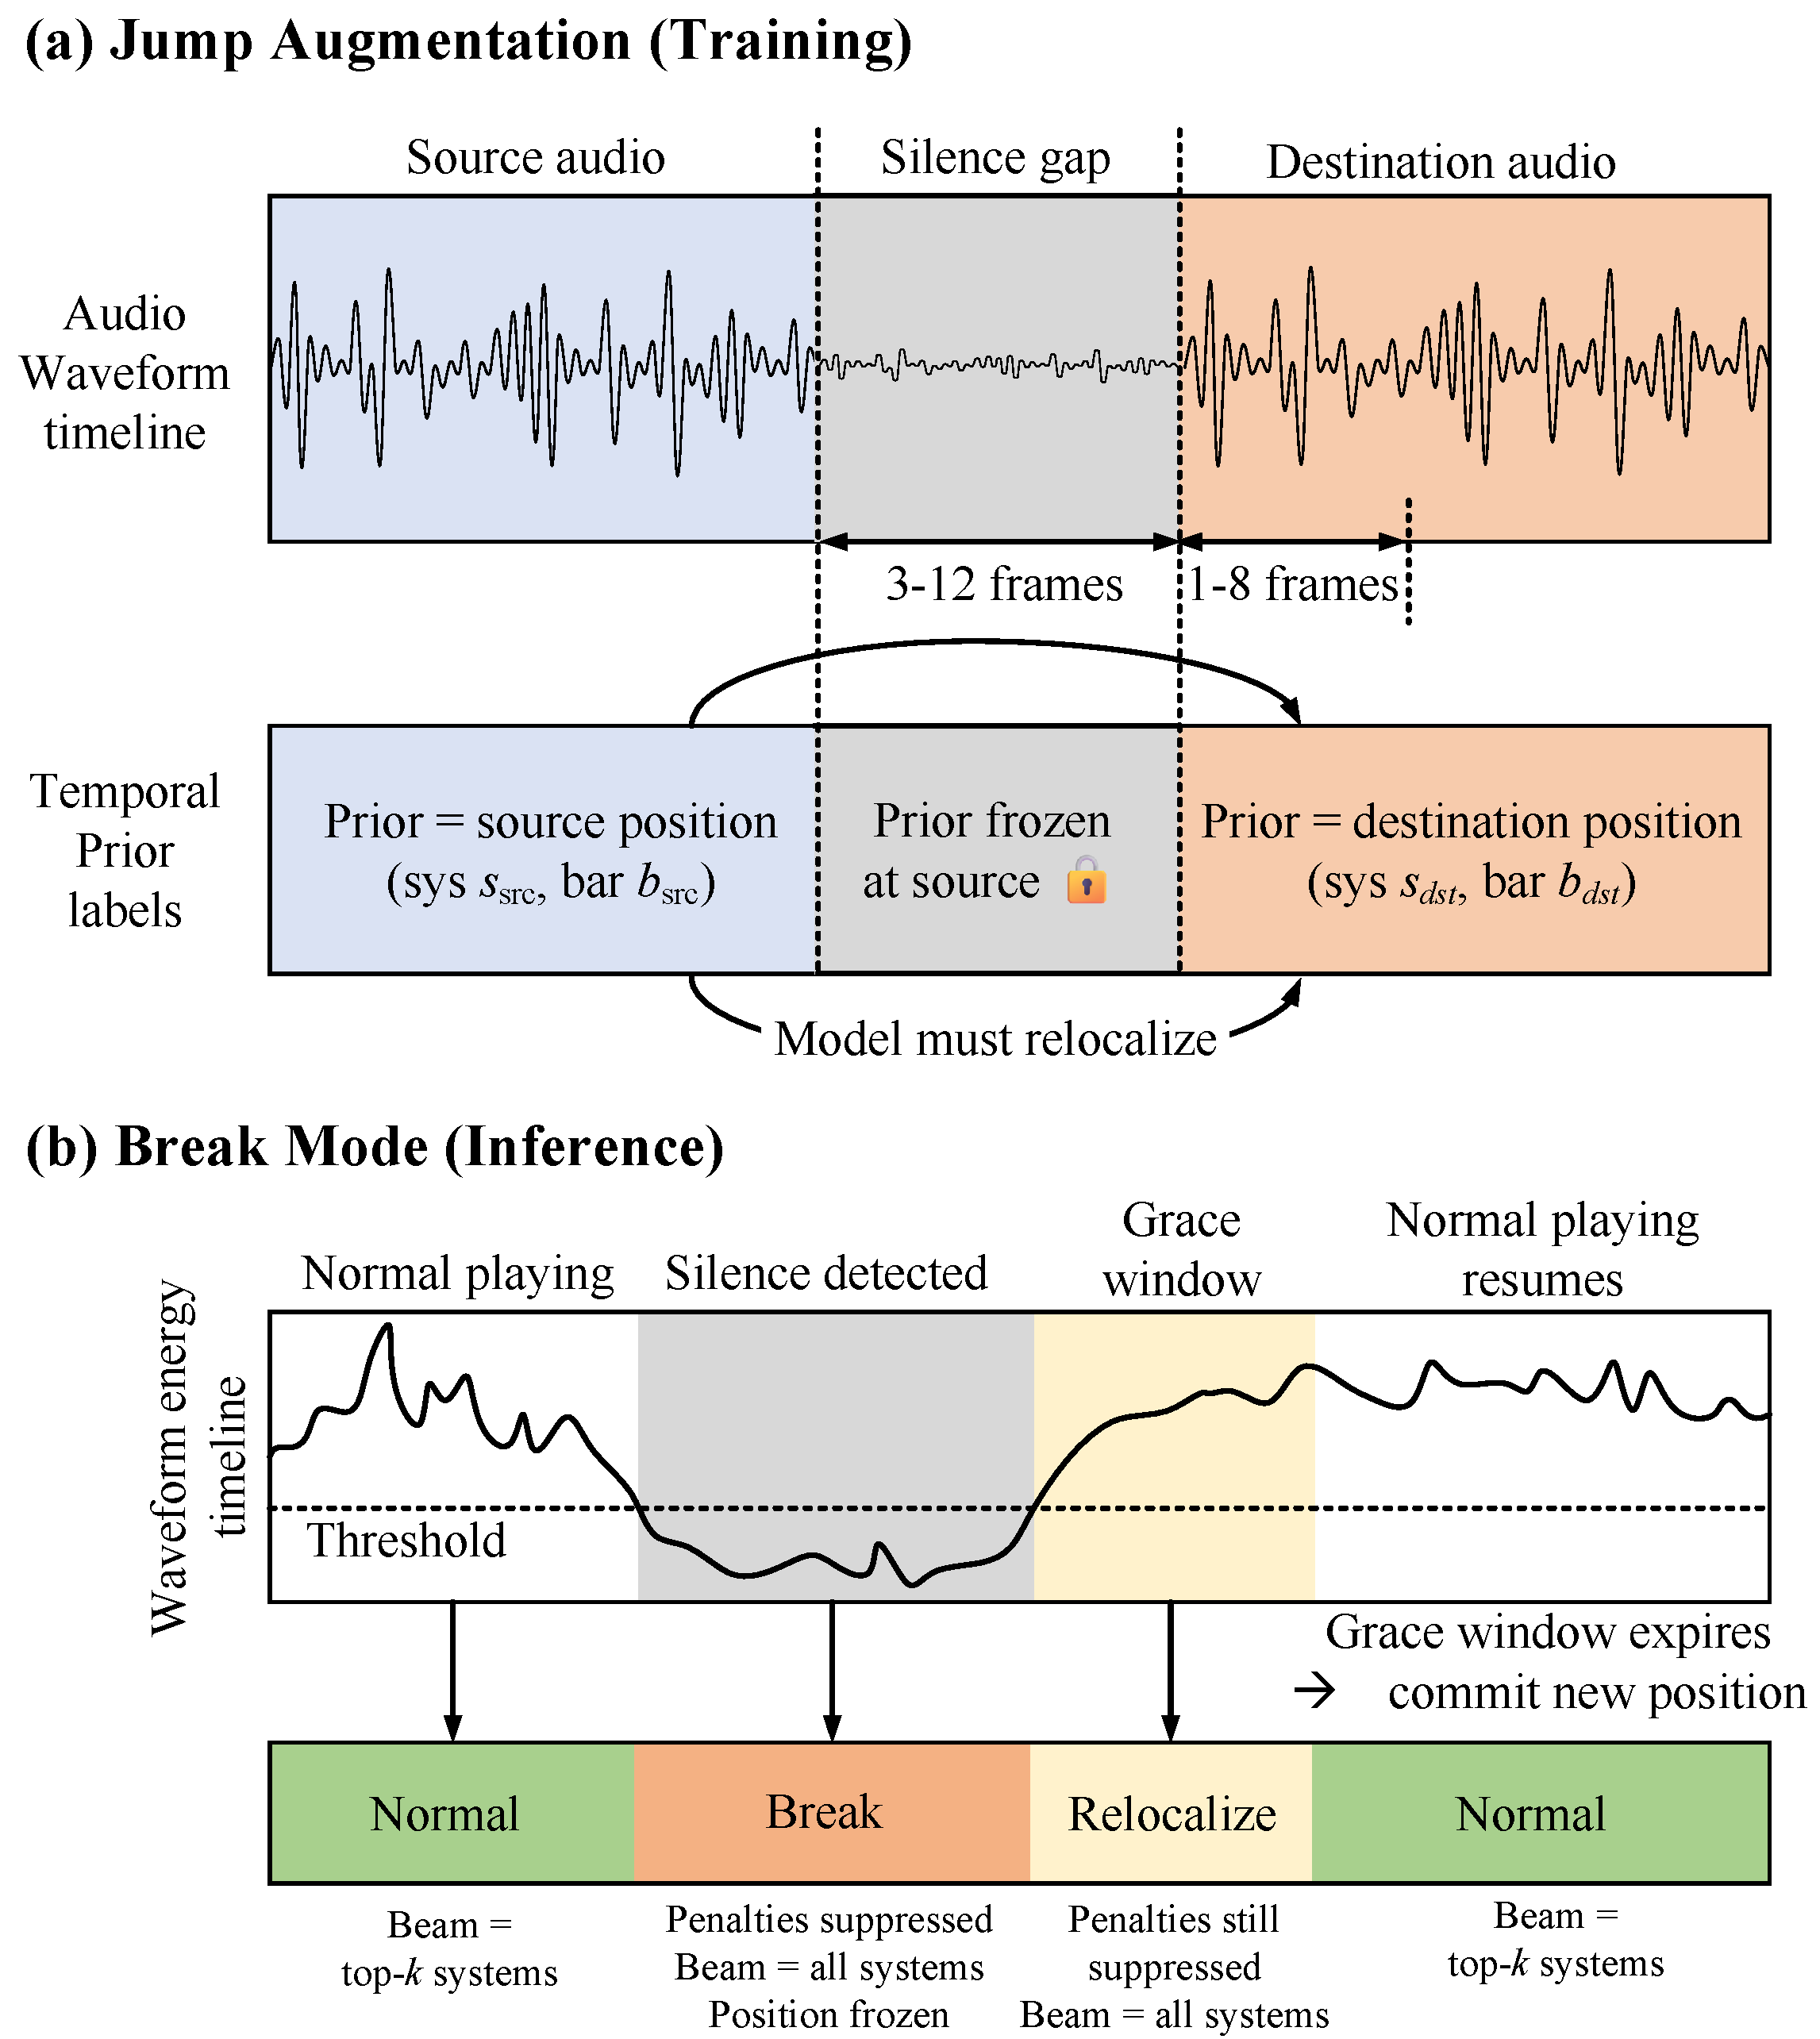
\includegraphics[width=\columnwidth]{figures/jump_recovery.pdf}
\caption{Jump recovery mechanism. (a)~Jump augmentation during training. (b)~Break mode at inference.}
\label{fig:jump_recovery}
\end{figure}

The jump-augmented training is illustrated in Figure~\ref{fig:jump_recovery}(a). Jump augmentation splices each sample with a controllable probability: a short silence (3--12 frames) is inserted, followed by audio from a randomly selected destination on the same or a different page. For same-page jumps, the previous system and bar labels are frozen at the source position, forcing the model to relocalize from audio evidence against a biased temporal prior.
 
At inference time, the break mode monitors waveform energy using a hysteresis rule. As presented in Figure~\ref{fig:jump_recovery}(b), when energy stays below a threshold for several consecutive frames, the tracker enters a break state: transition penalties are suppressed, the system beam is widened to cover all candidates, and the committed position is frozen. When energy rises again, penalties remain suppressed for a short grace window during which the tracker relocalizes to the jump destination. The Mamba hidden state is preserved throughout, maintaining temporal continuity across the silence gap.

